\chapter{Theory} \label{Chapter:Theory}

This chapter is about the literature review that will serve as a valuable background for future research.



\section{Defining video game genres}

The first attempts to classify video games occurred years after the first video game was released. In his book published in 1984, Chris Crawford listed games in two major categories, namely skill and action games (S\&A) which rely heavily on hand-eye coordination and motor skills and are usually fast-paced, and strategy games that emphasize more decision-making, and due to their nature, they generally take longer than S\&A games\cite{crawford1984art}. Within these main categories, Crawford defined multiple subdivisions for finer categorization. Some of these categories have evolved into modern game genres and are still present today, like sports and adventure games, while others, including paddle games, D\&D games and games of chance have completely merged into other genres and do not exist on their own. It is important to note that Crawford did not refer to these categories as genres.

Many of the first definitions of true video game genres were formulated by Mark J. P. Wolf, who also compared video games with the other existing media types, but mainly cinema \cite{wolf2002genre}. He concluded that video games and movies, while many similarities exist, can not be categorized the same way, due to their differences in interactivity (video games require active participation from the audience). Thus, the 41 genres and subgenres explained in his paper\cite{wolf2002genre} are based on interactivity aspects, instead of iconography. The border between some of these genres is blurry, Racing and Driving, Catching and Capturing, Obstacle Course, and Platform all have a surprisingly similar definition to the other, differing only in a few parameters; however, these similarities are explicitly stated by the author.

Another approach was made in 2006 by Thomas H. Apperley, who agreed with Wolf that games cannot be categorized like other media types. He also criticized earlier game categorization attempts, mainly because they are "loose aesthetic clusters based around video games' aesthetic linkages to prior media forms"\cite{apperley2006genre}. Instead, his proposed framework tries to shape a new set of genres around the style of "ergodic interaction" that takes place within the games. In his paper, he defined four distinct video game genres. \textit{Simulation} games mimic the intricate processes of real-life systems, such as cars or cities. \textit{Strategy} games, including real-time strategy (RTS) and turn-based strategy (TBS), are outliers due to their similarity to board games. These games usually have a god's-eye view and information-heavy interfaces. \textit{Action} games include first-person shooters (FPS) and third-person games and focus more on the player's performance in combat manoeuvres and aiming with weapons, and unlike strategy games, they do not contain complex decision-making processes. And finally, \textit{role-playing} games (RPG), often compared to pencil-and-paper RPGs such as Dungeons and Dragons, usually revolve around fantasy themes and focus on some form of character development, such as the collection of experience or skill points.

The early video game taxonomies were not applicable to the modern genres that followed\cite{starosta2024tangled}. Such complex genres as Massively Multiplayer Online Role-Playing Games (MMORPG) or Multiplayer Online Battle Arenas (MOBA) could not fit into the existing categories that were shaped, as they are a mix of several already defined game types (Multiplayer and Role-Playing).

Overall, it can be observed that the video game industry is and has always been struggling to come up with a universal organization system for games. Existing categorization methods, such as those used for books or movies, could not be applied due to differences between the mediums\cite{lee2014facet}.

Instead of sticking to one taxonomy, Steam\cite{steam}, an online video game store, uses a list of predefined, as well as user-defined tags (consisting of one or a few words) to categorize games published on the platform. Tags are similar, and sometimes identical, to the name of genres discussed in the above-mentioned papers, however, there is no definition linked to them. What each tag means is determined by the types of games assigned to them on the platform. This enables greater freedom in video game categorization than sicking to a chosen taxonomy would, since tags can expand and adapt to new game types, while taxonomies remain the same.



\section{Finding genre combinations}

Today's most popular game store on PC, Steam\cite{steam}, which, at the time of writing, has a library of over 204.000 apps, including the majority of modern video games. There are some exceptions, however, as some games are platform-specific and thus have never been released on Steam, but the number of such games can only be measured in the hundreds, so they will be considered insignificant for this research.

Steam uses two systems to categorize this massive amount of content. First, developers and publishers pick from a list of pre-defined genres to assign to their apps during upload. Second, users who download these apps can assign them user-defined tags that can indicate genre, theme, aesthetics, or even difficulty, and help other users find new apps that are to their liking. From the user's point of view, only the tags are visible on the apps' dedicated pages while genres are only used as filtering in the store's search field.

Steam has a public API (Application Programming Interface) that can be used to query data about their games and apps. This API, however, is not well-documented, thus it would take a considerable amount of trial and error to use it properly. Luckily, a relatively fresh dataset\cite{steamCatalogInsight2024} can be found on GitHub that, according to the author, was acquired in October 2024 using the Steam API and contains all the data necessary to find existing genre combinations on Steam. To check exactly how up-to-date this data set is, I checked the number of games under some tags on Steam and compared them with the numbers found in the data set, and the differences were around 40\%, which is unexpectedly high. However, games released in October 2024 can be found in the data set as expected with the correct release dates, indicating the data was truly acquired in or after October 2024. The explanation for such a large difference in the numbers could be explained by the ever-rising number of new games published each month on the platform and the new tags applied to games during this two-month period. However, the ratio between the tag occurrences could not change significantly in such a short time. These data are in CSV format which is mostly used by spreadsheet editors such as Excel or Numbers, but can easily be read from script too.

Going through the data set and individually counting the times each tag occurs, it is easy to determine that Steam currently uses 447 tags and 121 genres. It can also be observed that tag occurrences, as seen in figure \ref{figure:tags}, like many other data sets, seem to follow Zipf's law loosely\cite{li2002zipf}. Interestingly, some of the tags make little sense, like "Intentionally Awkward Controls" or "TrackIR", and do not represent a genre, but rather some other aspect of the game. There are a few tags like "Warhammer 40K" that solely indicate which franchise the game belongs to.

\begin{figure}[h]
    \centering
    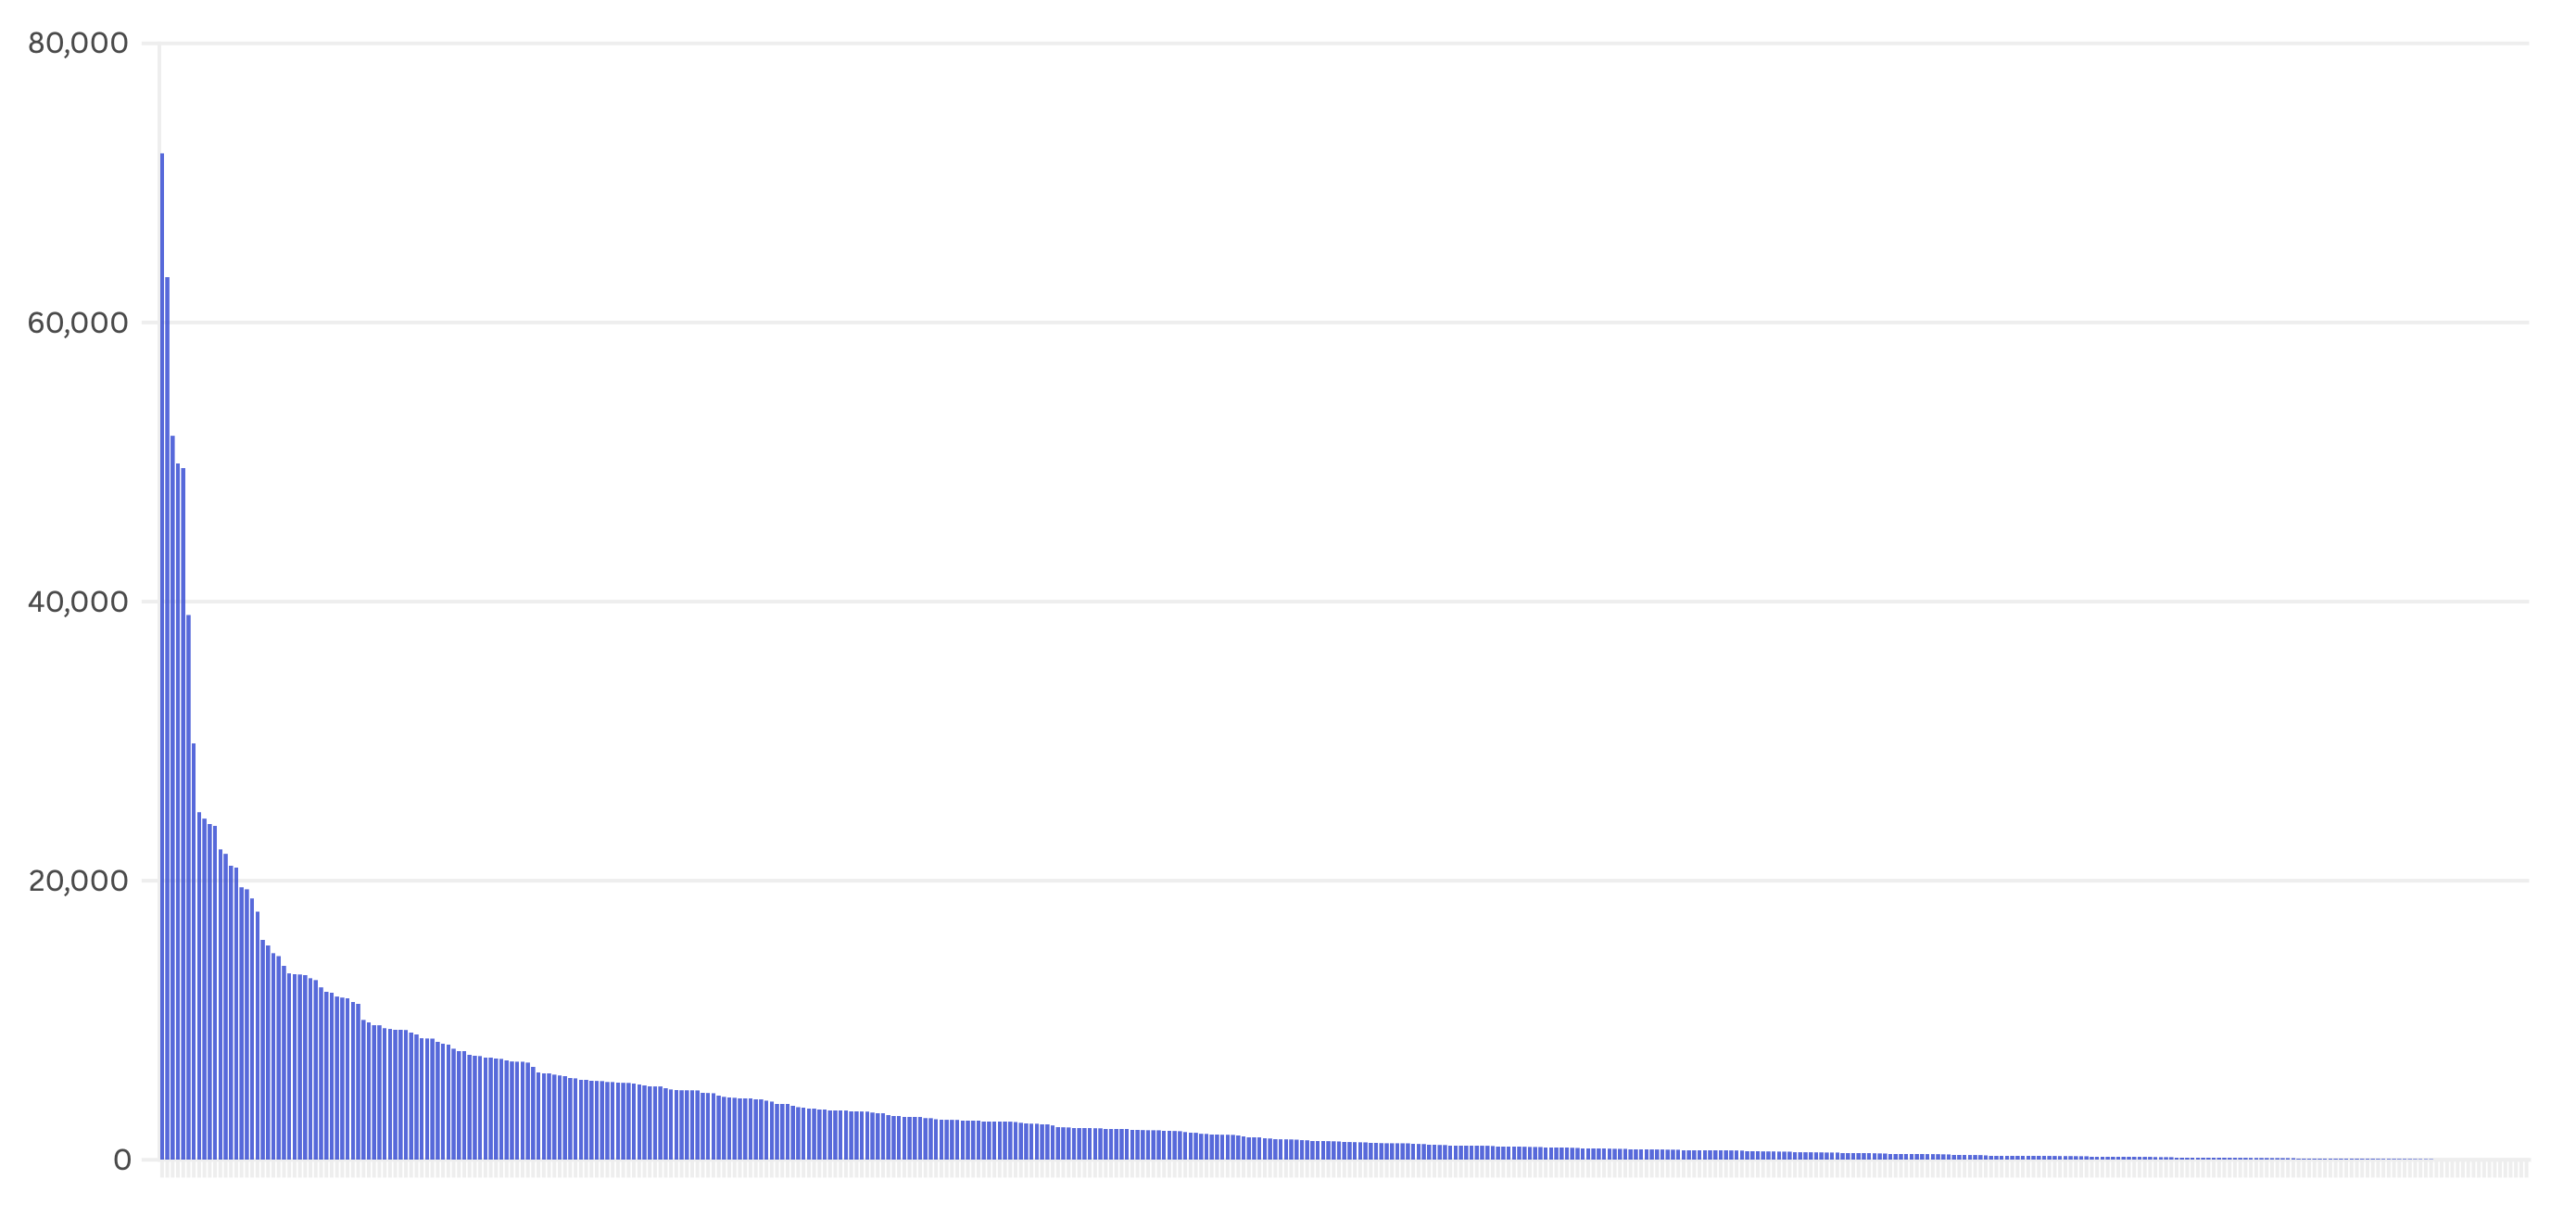
\includegraphics[width=\textwidth]{images/tag-occurrences.png}
    \caption{Tag occurrences}
    \label{figure:tags}
\end{figure}

On the other hand, the genre distribution in figure \ref{figure:genres} seems unbalanced. The reason for that is that for some reason, 84 of the 121 genres are localized versions of others, and each appears less than 30 times. These genres can be safely discarded, as their occurrence times would not contribute too much to the other numbers.

\begin{figure}[h]
    \centering
    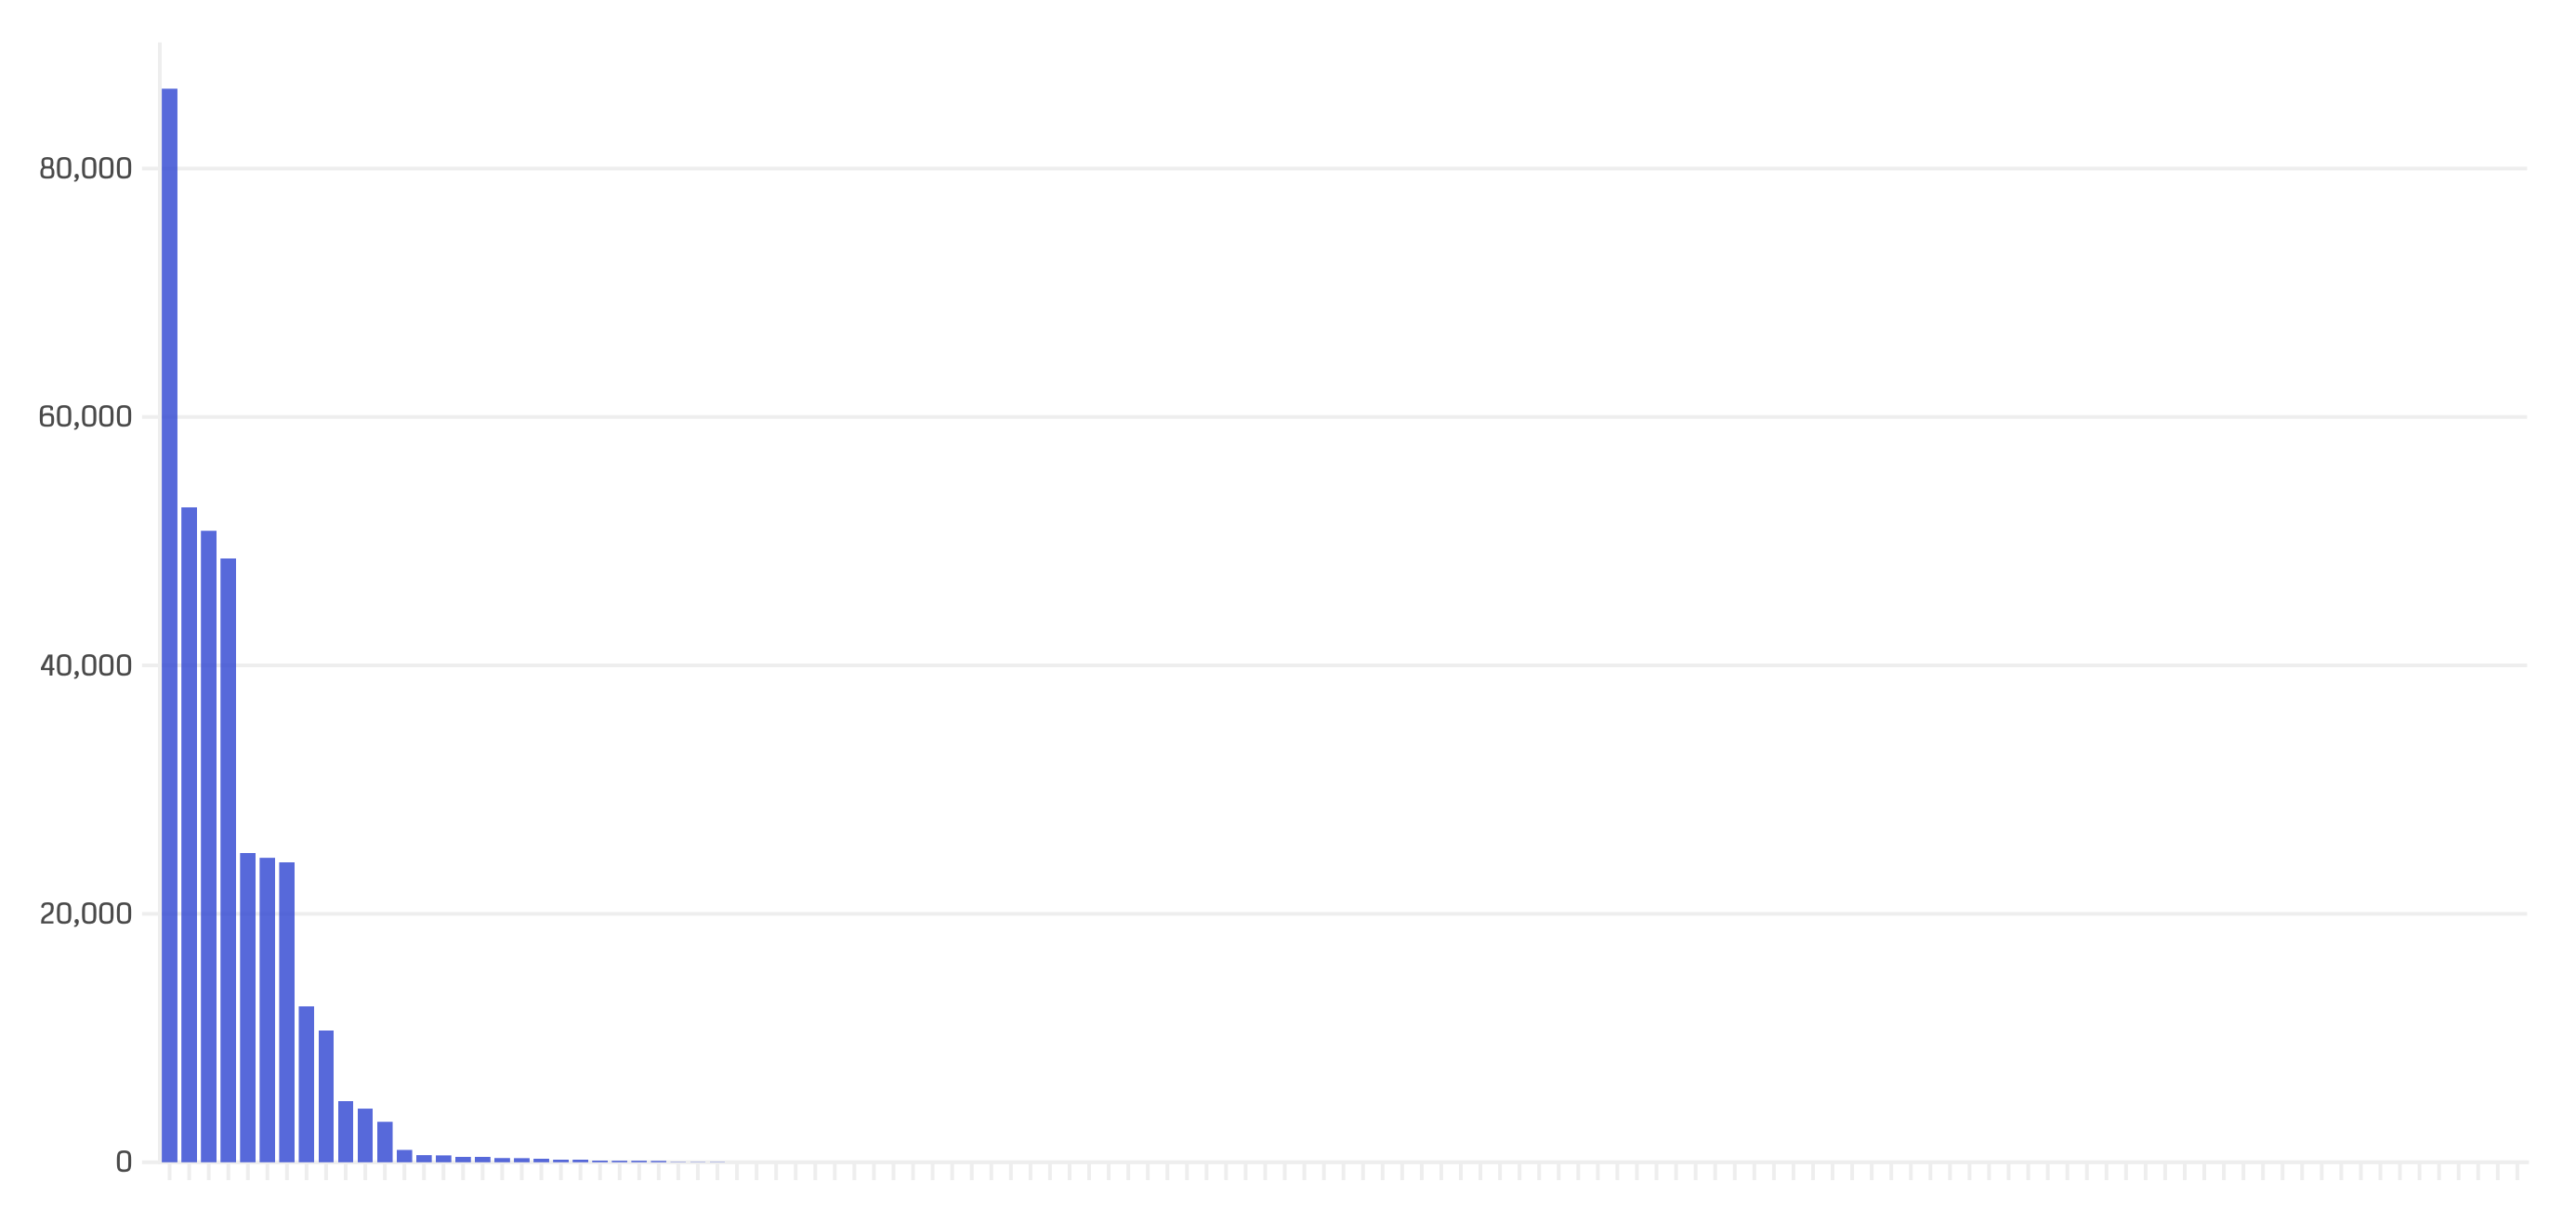
\includegraphics[width=\textwidth]{images/genre-occurrences.png}
    \caption{Genre occurrences}
    \label{figure:genres}
\end{figure}

However, since Steam uses only a handful of genres to categorize games, these genres are vague. Therefore, for this thesis, I will use Steam tags instead, as tags provide a much finer way to describe what genres the developed game prototype should belong to and what types of game mechanics they use.

It is important to note that the dataset's author also looked for genre combinations as seen in figure \ref{figure:genre-pairs}, but they only used combinations of two genres, while I was more interested in more complex mixtures. Furthermore, they only included tags assigned to at least 900 games in the Steam library, and that criteria takes away almost half of the tags. For this thesis, I was interested in the other half of the tags, those that are used rarely but at the same time clearly represent a genre or sub-genre. To extract exactly the data I needed, I had to write my own script which will be discussed in chapter \ref{Chapter:Planning}.

\begin{figure}[h]
    \centering
    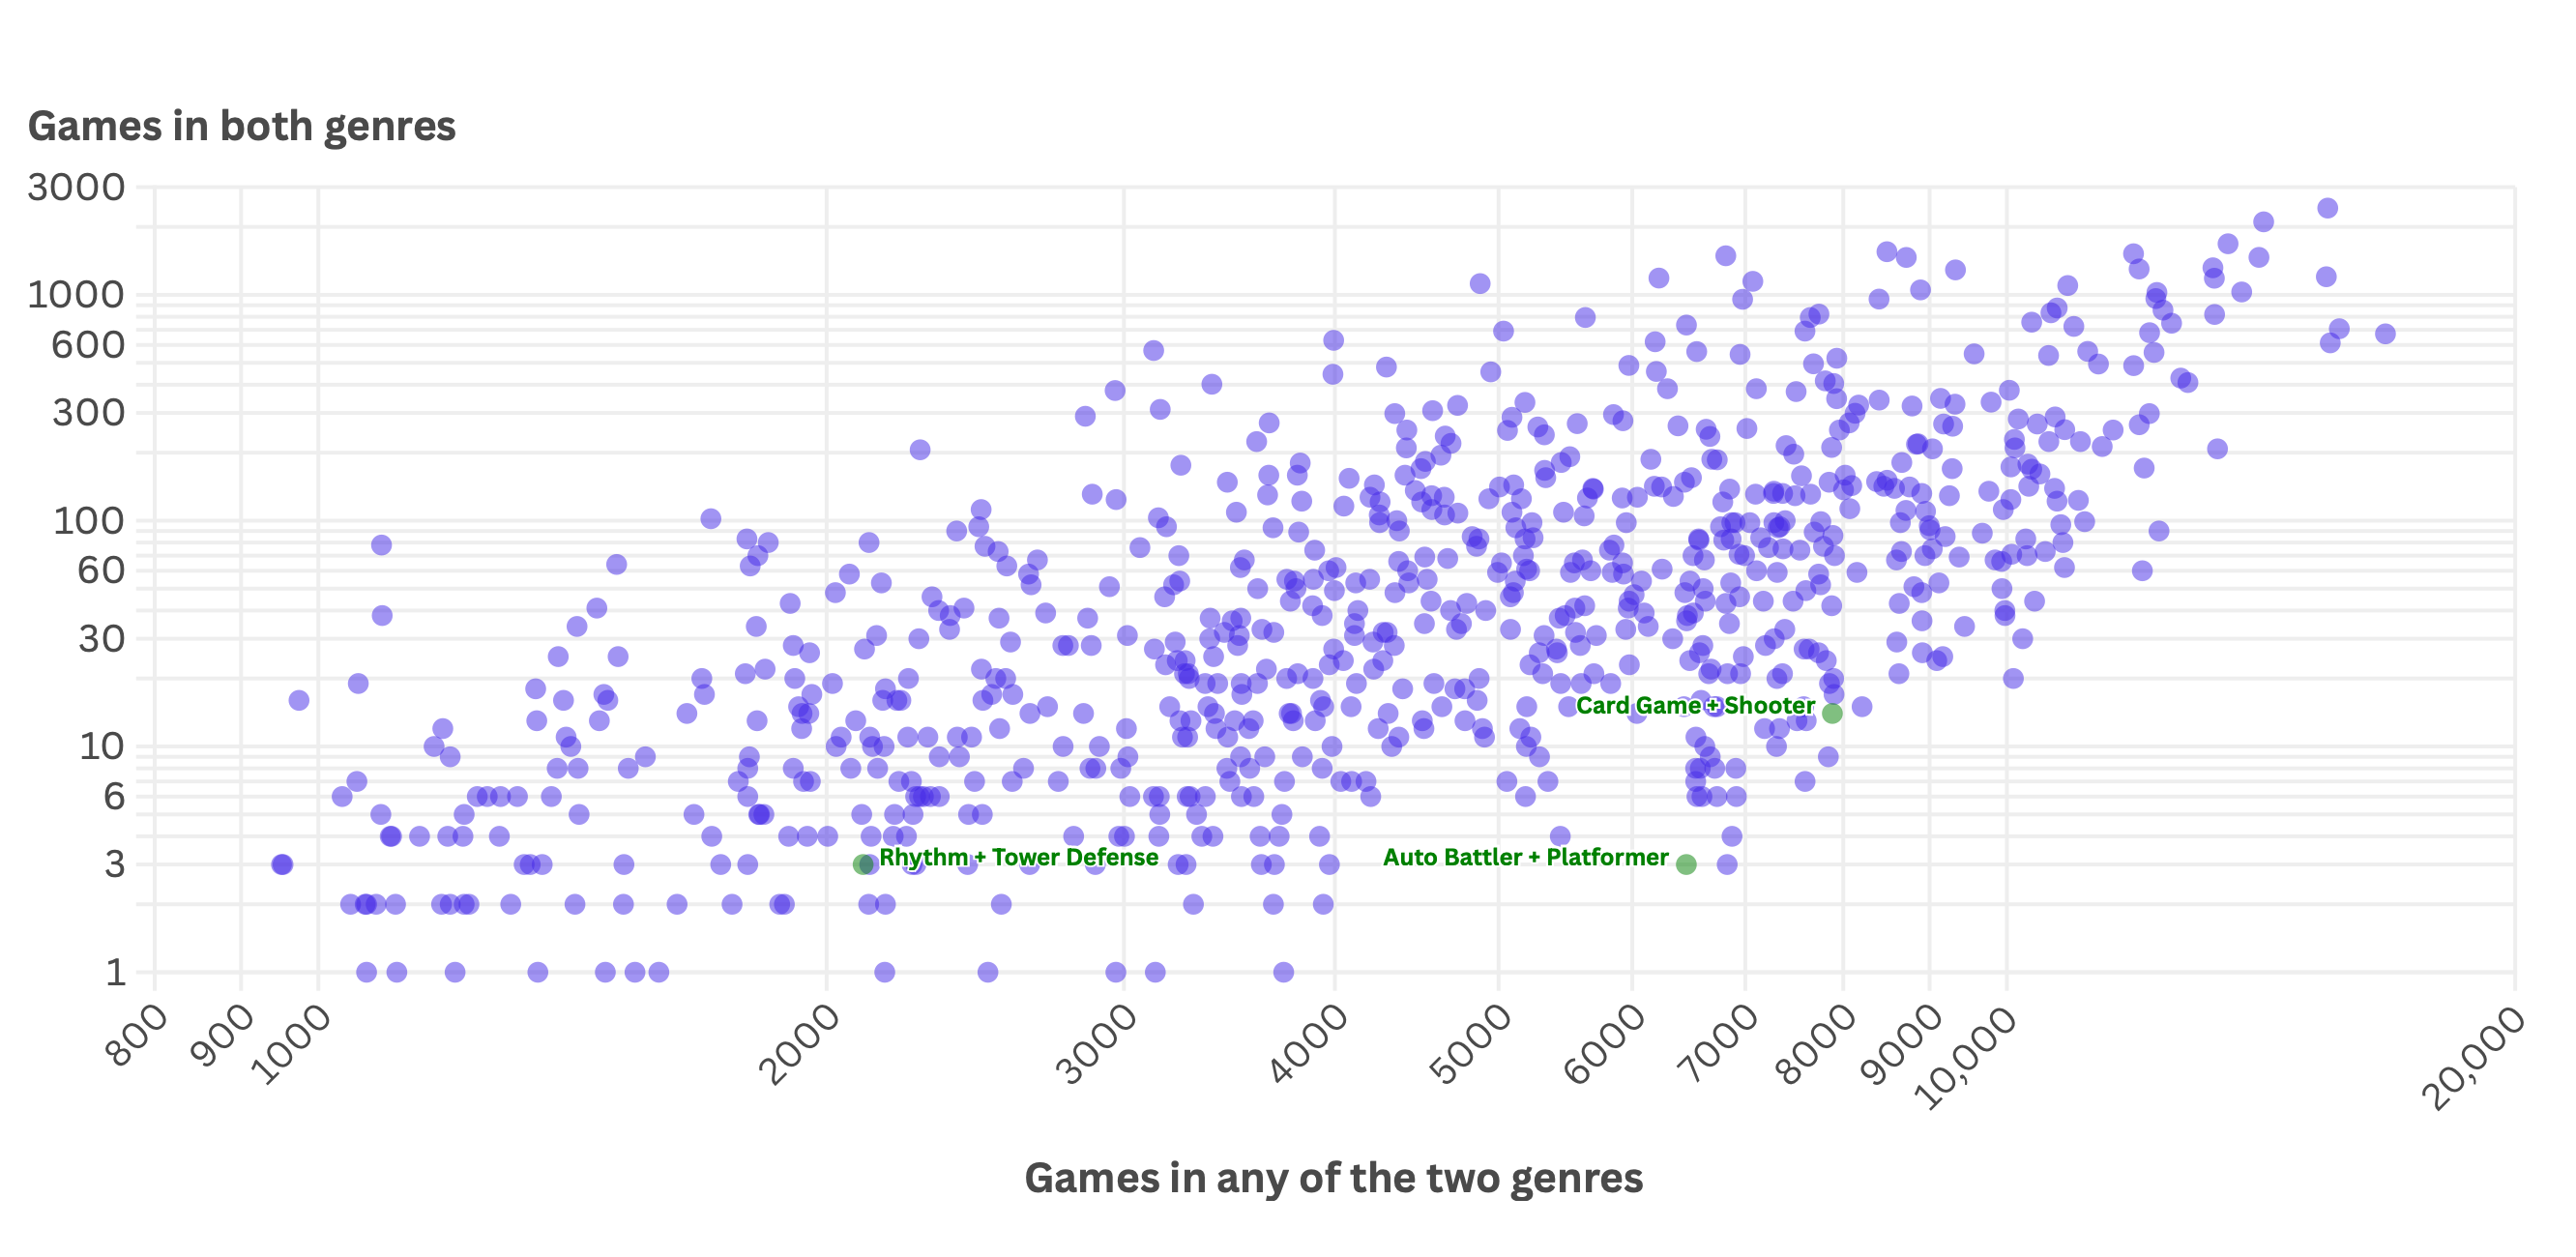
\includegraphics[width=\textwidth]{images/genre-pairs.png}
    \caption{Most frequent genre pairs}
    \label{figure:genre-pairs}
\end{figure}



\section{Game engines}

This thesis will include the development of a game prototype, and to reduce development time, a game engine will be used. There are many freely available game engines on the market at the time this thesis is being written, so to pick one, a short comparison needs to be made.

But first of all, what is a game engine? To answer this question, it would be a good idea to look back at the very first game engine. Doom Engine was developed for Doom (1993) by id Software, it was the first of its kind \cite{gregory2018gameEngineArchitecture}, the very first piece of software that had its components well-defined and separated, allowing developers to make different games with minimal modifications made to the game engine itself. Soon many major game development studios started to develop their own game engines, while licensing other's already working engines started to become a norm.

Developers today can also choose to use free-to-use game engines such as Unreal Engine \cite{unrealEngine} or Unity \cite{unity}. These engines are usually for general purposes, meaning that they include a handful of features that make it possible to develop any kind of video game with them, with the side-effect of being hard to learn on a professional level. Additionally, they are not entirely free, as there is usually a limit above which developers have to start paying a share of their total revenue to the engine. 

There are more compact alternatives, such as Godot\cite{godot} or LÖVE\cite{love2d}, which are completely free and open-source, meaning that developers can actively contribute to their code base to implement new features. However, they often lack features found in more robust engines.



\section{Game development} \label{Section:GameDevelopment}

Creating video games is a combination of several professions. It includes programming, game design, asset creation such as sprites, 3D models, music and sound effects, and even marketing. Dedicated tools can be used for each of these areas; some of them are discussed in Axel Ljungdahl's master's thesis \cite{ljungdahl2020individual} on individual game development. Axel's work is considered extremely valuable regarding this thesis, as it provides important tips and guidelines for how a game prototype should be developed individually, using only affordable tools.

For programming, code editors, or IDEs (Integrated Development Environments) can be used to help with coding syntax, formatting, and debugging, as well as code completion. Popular options include Visual Studio\cite{visualStudio}, Visual Studio Code\cite{visualStudioCode} and the JetBrains\cite{jetBrains} suite. Some game engines, such as Godot, even have their own integrated code editors. \cite{ljungdahl2020individual}

For creating graphical assets, like sprites or textures, one can choose between raster graphics, storing images as a grid of rectangular pixels, and vector graphics, storing images as mathematical models that can be scaled without using detail. Respectively, free tools such as GIMP \cite{gimp} and Figma \cite{figma} can be used for these approaches. If the game is three-dimensional, it usually requires 3D model assets, which can be created using Blender\cite{blender}. \cite{ljungdahl2020individual}

Music and sound effects can be created with free tools such as LLMS. Existing audio files can be edited using Audacity. Audio can also be recorded using a regular microphone found inside an average smartphone or laptop. Some games, like Samorost 3\cite{samorost3_2016}, use sound effects produced solely by mouth and real instruments.